\documentclass[12pt,letterpaper]{report}
% Preámbulo compartido para los documentos del Sistema de Solicitudes (UAZ).
% Identidad visual alineada con el SRS. Compilar con pdflatex.
\usepackage[utf8]{inputenc}
\usepackage[T1]{fontenc}
\usepackage[spanish, mexico]{babel}
\usepackage{geometry}
\geometry{left=2.5cm, right=2.5cm, top=2.5cm, bottom=2.5cm}
\usepackage{graphicx}
\usepackage{float}
\usepackage{longtable}
\usepackage{tabularx}
\usepackage{array}
\usepackage{booktabs}
\usepackage{hyperref}
\usepackage{enumitem}
\usepackage{xcolor}
\usepackage{fancyhdr}
\usepackage{titlesec}
\usepackage{caption}
\usepackage{listings}

\definecolor{uazblue}{RGB}{0, 51, 102}
\definecolor{lightgray}{RGB}{240, 240, 240}
\definecolor{codebg}{RGB}{248, 248, 248}

\hypersetup{colorlinks=true, linkcolor=uazblue, urlcolor=uazblue, citecolor=uazblue}

\newcolumntype{L}[1]{>{\raggedright\arraybackslash}p{#1}}
\newcolumntype{C}[1]{>{\centering\arraybackslash}p{#1}}
\newcolumntype{R}[1]{>{\raggedleft\arraybackslash}p{#1}}

\titleformat{\chapter}[display]
  {\normalfont\huge\bfseries\color{uazblue}}{\chaptertitlename\ \thechapter}{20pt}{\Huge}
\titlespacing*{\chapter}{0pt}{-20pt}{40pt}

\lstset{
  basicstyle=\ttfamily\footnotesize,
  backgroundcolor=\color{codebg},
  frame=single,
  rulecolor=\color{lightgray},
  breaklines=true,
  columns=fullflexible,
  showstringspaces=false,
  keepspaces=true,
}

% Portada institucional reutilizable:
% \portada{TÍTULO DEL DOCUMENTO}{Subtítulo opcional}
\newcommand{\portada}[2]{%
\begin{titlepage}
    \centering
    \vspace*{1cm}
    {\Large\bfseries UNIVERSIDAD AUTÓNOMA DE ZACATECAS}\\[12pt]
    {\normalsize UNIDAD ACADÉMICA DE INGENIERÍA ELÉCTRICA}\\[24pt]
    \IfFileExists{uaz.png}{
\includegraphics[width=1.5in]{uaz.png}\\[40pt]}{\vspace{40pt}}
    {\large\bfseries #1}\\[6pt]
    {\large\bfseries SISTEMA DE SOLICITUDES}\\[10pt]
    {\normalsize #2}\\[24pt]
    {\normalsize\bfseries
    Diego Iván Correa Navarrete\\
    Juan Antonio González del Río\\
    Diego Arturo Ramos Ávila\\
    Ángel David Carlos Silva\\}
    \vspace{30pt}
    {\normalsize\bfseries LICENCIATURA EN INGENIERÍA DE SOFTWARE}\\[16pt]
    {\normalsize Junio de 2026}
\end{titlepage}}

\begin{document}
\portada{DOCUMENTO DE DISEÑO DE SOFTWARE (SDD)}{}
\tableofcontents\newpage

% =====================================================================
\chapter{Introducción}
% =====================================================================

\section{Propósito}

Este documento describe el diseño del software (\textit{Software Design
Description}, SDD) del \textbf{Sistema de Solicitudes} de la Universidad
Autónoma de Zacatecas (UAZ). Su objetivo es traducir los requerimientos
funcionales y no funcionales descritos en la Especificación de Requerimientos
de Software (SRS) a una arquitectura concreta, una descomposición en módulos,
un modelo de datos y un conjunto de decisiones de diseño que guíen la
construcción, prueba y mantenimiento del sistema.

El SDD está dirigido a las personas que implementan, prueban, revisan o
mantienen el sistema: equipo de desarrollo, responsables de aseguramiento de
calidad y personal de operación. Presupone familiaridad con Python, Django y
los conceptos de arquitectura por capas.

\section{Alcance}

El Sistema de Solicitudes es una aplicación web monolítica que digitaliza la
gestión de solicitudes académicas y administrativas de la UAZ, reemplazando
procesos manuales basados en papel y correo por un flujo trazable. El sistema
permite que estudiantes y docentes presenten solicitudes mediante formularios
dinámicos configurables, da seguimiento al ciclo de vida de cada solicitud
mediante una máquina de estados, genera documentos PDF a partir de plantillas,
notifica por correo a las partes involucradas y ofrece administración del
catálogo, gestión de archivos adjuntos, atención por roles y reportes
agregados.

El sistema delega la autenticación a un proveedor externo (recibe un token JWT)
y consulta datos de usuario al sistema institucional SIGA. No procesa pagos:
únicamente recibe comprobantes como archivos adjuntos.

\section{Definiciones, acrónimos y abreviaturas}

\begin{longtable}{L{3.2cm} L{11cm}}
\toprule
\textbf{Término} & \textbf{Significado} \\
\midrule
\endhead
SDD & \textit{Software Design Description}: documento de diseño del software. \\
SRS & \textit{Software Requirements Specification}: especificación de requerimientos. \\
DTO & \textit{Data Transfer Object}: objeto inmutable que transporta datos entre capas. \\
ORM & \textit{Object-Relational Mapping}: capa de mapeo objeto-relacional de Django. \\
ABC & \textit{Abstract Base Class}: clase base abstracta (interfaz) de Python. \\
DI & \textit{Dependency Injection}: inyección de dependencias. \\
JWT & \textit{JSON Web Token}: token firmado emitido por el proveedor de autenticación. \\
SIGA & Sistema de Información para la Gestión Académica de la UAZ. \\
CSP & \textit{Content Security Policy}: política de seguridad de contenido HTTP. \\
Folio & Identificador único de una solicitud con formato \texttt{SOL-AAAA-NNNNN}. \\
Plantilla & Documento HTML+CSS administrable que se renderiza a PDF. \\
Snapshot & Fotografía inmutable de la definición de campos al crear una solicitud. \\
RF / RNF & Requerimiento funcional / requerimiento no funcional. \\
\bottomrule
\end{longtable}

\section{Referencias}

\begin{itemize}[leftmargin=1.4em]
  \item Especificación de Requerimientos de Software (SRS) del Sistema de Solicitudes.
  \item \texttt{specs/global/architecture.md} — arquitectura global (fuente principal de este diseño).
  \item \texttt{specs/global/requirements.md} — requerimientos funcionales (RF) y no funcionales (RNF).
  \item \texttt{specs/apps/*/design.md} — diseño detallado por funcionalidad.
  \item \texttt{.claude/rules/django-code-architect.md} — reglas arquitectónicas canónicas.
  \item Diagrama entidad-relación: \texttt{entregables/documentos/esquema\_bd\_diagrama.pdf}.
\end{itemize}

\section{Panorama del documento}

El Capítulo~2 describe la arquitectura del sistema y el flujo de una petición.
El Capítulo~3 descompone el sistema en aplicaciones y funcionalidades. El
Capítulo~4 presenta el modelo de datos y el diagrama entidad-relación. El
Capítulo~5 documenta las decisiones de diseño y los patrones aplicados. Los
Capítulos~6, 7 y 8 cubren el diseño de interfaz de usuario, la seguridad y las
tecnologías y dependencias, respectivamente.

% =====================================================================
\chapter{Arquitectura del sistema}
% =====================================================================

\section{Estilo arquitectónico}

El sistema sigue un estilo \textbf{Vista $\rightarrow$ Servicio $\rightarrow$
Repositorio} (\textit{View $\rightarrow$ Service $\rightarrow$ Repository}),
con objetos de transferencia de datos (DTO) tipados con \textbf{Pydantic v2} en
cada frontera entre capas. Es una aplicación \textbf{monolítica} con
\textbf{plantillas renderizadas en el servidor} (Django Templates con Tailwind
CSS v4 y Alpine.js v3); deliberadamente \textbf{no} expone una API REST con
DRF.

Cada capa tiene una responsabilidad única y bien delimitada:

\begin{itemize}[leftmargin=1.4em]
  \item \textbf{Vista (Vista, frontera HTTP).} Posee las preocupaciones HTTP:
  recibe la petición, resuelve el actor a partir del JWT, instancia el formulario,
  traduce \texttt{cleaned\_data} a un DTO de entrada, invoca el servicio y
  renderiza la plantilla o emite la redirección. Nunca llama directamente a un
  repositorio ni al ORM.
  \item \textbf{Formulario.} Analiza y valida la entrada del usuario y convierte
  \texttt{cleaned\_data} en un DTO de Pydantic antes de cruzar hacia el servicio.
  \item \textbf{Servicio (lógica de negocio).} Python puro, definido como una
  clase base abstracta (ABC) más su implementación. Contiene la lógica de
  dominio, la autorización por política (p.\,ej. ``solo el dueño edita'') y la
  orquestación transaccional. No conoce HTTP ni el ORM.
  \item \textbf{Repositorio (acceso a datos).} Único lugar donde vive el ORM de
  Django. Definido como ABC más implementación. Recibe y devuelve DTOs; traduce
  toda excepción de Django (\texttt{Model.DoesNotExist}) a una excepción de
  dominio antes de que escape de la capa.
\end{itemize}

\begin{table}[H]
\centering
\caption{Capas y su responsabilidad (de la frontera HTTP hacia la base de datos).}
\begin{tabularx}{\textwidth}{L{3.2cm} X L{3.6cm}}
\toprule
\textbf{Capa} & \textbf{Responsabilidad} & \textbf{Conoce} \\
\midrule
Vista        & HTTP, autorización por rol (mixins), renderizado de plantillas. & Formularios, Servicios \\
Formulario   & Parseo y validación de entrada; producción de DTO. & Schemas (DTO) \\
Servicio     & Lógica de negocio, autorización por política, transacciones. & Repositorios, otros Servicios (vía interfaz) \\
Repositorio  & Consultas y escrituras ORM; traducción a DTO y a excepciones. & ORM, Modelos \\
ORM / BD     & Persistencia en PostgreSQL (SQLite en pruebas internas). & --- \\
\bottomrule
\end{tabularx}
\end{table}

\section{Flujo de una petición}

El recorrido de una petición autenticada atraviesa las capas de forma
descendente y regresa por la misma ruta con DTOs:

\begin{enumerate}[leftmargin=1.6em]
  \item La petición HTTP entra por el \texttt{RequestIDMiddleware}, que asigna
  un identificador de correlación, y por el \texttt{JwtAuthenticationMiddleware},
  que valida el token (cookie \texttt{stk} o cabecera \texttt{Authorization: Bearer}),
  fija \texttt{request.user} y \texttt{request.user\_dto}.
  \item La \textbf{Vista} aplica los \textit{mixins} de permiso
  (\texttt{LoginRequiredMixin}, mixins por rol), construye el formulario con
  \texttt{request.POST}/\texttt{request.FILES} y lo valida.
  \item El \textbf{Formulario} produce un \textbf{DTO de entrada} de Pydantic a
  partir de \texttt{cleaned\_data}.
  \item La Vista invoca al \textbf{Servicio} pasándole el DTO y el actor
  (\texttt{UserDTO}).
  \item El \textbf{Servicio} ejecuta la lógica de dominio y delega la persistencia
  al \textbf{Repositorio} dentro de \texttt{transaction.atomic()} cuando aplica.
  \item El \textbf{Repositorio} ejecuta el ORM y devuelve un \textbf{DTO de salida}.
  \item El Servicio devuelve el DTO a la Vista, que lo entrega a la plantilla para
  su renderizado en el servidor.
\end{enumerate}

\begin{table}[H]
\centering
\caption{Esquema textual del flujo de una petición.}
\begin{tabularx}{\textwidth}{X}
\toprule
\texttt{HTTP Request} \\
\quad$\downarrow$ \texttt{RequestIDMiddleware} $\rightarrow$ \texttt{JwtAuthenticationMiddleware} \\
\texttt{Vista (frontera HTTP)} --- Formulario (parsea + valida) $\rightarrow$ \texttt{DTO} \\
\quad$\downarrow$ \\
\texttt{Servicio (lógica de negocio, ABC + impl.)} \\
\quad$\downarrow$ \\
\texttt{Repositorio (solo ORM, ABC + impl.)} $\rightarrow$ \texttt{DTO} \\
\quad$\downarrow$ \\
\texttt{Django ORM / PostgreSQL} \\
\bottomrule
\end{tabularx}
\end{table}

\section{Manejo de errores}

Todas las excepciones de dominio heredan de \texttt{\_shared.exceptions.AppError},
que centraliza los \textit{centinelas} reutilizables: \texttt{NotFound} (404),
\texttt{Conflict} (409), \texttt{Unauthorized} (403),
\texttt{AuthenticationRequired} (401), \texttt{DomainValidationError} (422) y
\texttt{ExternalServiceError} (502). Cada excepción concreta de una funcionalidad
es subclase de uno de estos centinelas y declara su \texttt{code} y su
\texttt{user\_message} en español.

El \texttt{AppErrorMiddleware} actúa como red de seguridad: en
\texttt{process\_exception} captura cualquier \texttt{AppError}, mapea el estado
HTTP correspondiente, registra el evento junto con el \texttt{request\_id} y
renderiza \texttt{\_shared/error.html} (o devuelve JSON para peticiones AJAX).
Las vistas pueden capturar \texttt{AppError} selectivamente para devolver
\texttt{field\_errors} al formulario y re-renderizarlo con las marcas de error.

\begin{table}[H]
\centering
\caption{Centinelas de \texttt{AppError} y su estado HTTP.}
\begin{tabularx}{\textwidth}{L{5.2cm} L{2.2cm} X}
\toprule
\textbf{Centinela} & \textbf{HTTP} & \textbf{Uso} \\
\midrule
\texttt{AuthenticationRequired} & 401 & Token ausente, inválido o expirado. \\
\texttt{Unauthorized}           & 403 & Rol o política de dominio no autorizada. \\
\texttt{NotFound}               & 404 & Recurso inexistente. \\
\texttt{Conflict}               & 409 & Transición de estado inválida, conflicto de unicidad. \\
\texttt{DomainValidationError}  & 422 & Validación de negocio fallida (con \texttt{field\_errors}). \\
\texttt{ExternalServiceError}   & 502 & SIGA o SMTP no responde. \\
\bottomrule
\end{tabularx}
\end{table}

\section{Reglas arquitectónicas transversales}

\begin{itemize}[leftmargin=1.4em]
  \item \textbf{El ORM nunca escapa del repositorio.} Solo el repositorio importa
  modelos y ejecuta \texttt{Model.objects}.
  \item \textbf{Dependencia entre funcionalidades.} Un servicio solo accede a los
  repositorios de su propia funcionalidad. Para leer datos de otra funcionalidad
  inyecta la \emph{interfaz de servicio} de esa funcionalidad, nunca su
  repositorio. Cuando el consumidor define la necesidad, declara un \emph{puerto}
  (ABC) y el productor provee el \emph{adaptador}.
  \item \textbf{DTOs en cada frontera.} Pydantic v2 para DTOs; nunca diccionarios
  desnudos cruzando capas.
  \item \textbf{Una clase pública por archivo.} Modelos, servicios y repositorios
  se definen uno por archivo.
  \item \textbf{Identificadores en inglés; texto al usuario en español.}
\end{itemize}

\section{Organización del proyecto}

El repositorio Git contiene en su raíz únicamente la infraestructura
(\texttt{Dockerfile}, \texttt{docker-compose.*.yml}, \texttt{Makefile},
\texttt{.env.example}). Todo el código Django vive dentro de \texttt{app/},
montado en \texttt{/app/} dentro del contenedor. Cada aplicación de Django es un
``corte vertical'' por capas; dentro de cada aplicación, cada funcionalidad
(\textit{feature}) es su propio paquete con esta estructura típica:

\begin{table}[H]
\centering
\caption{Estructura de paquete de una funcionalidad.}
\begin{tabularx}{\textwidth}{L{5.5cm} X}
\toprule
\textbf{Archivo / carpeta} & \textbf{Contenido} \\
\midrule
\texttt{schemas.py} & DTOs de Pydantic. \\
\texttt{exceptions.py} & Excepciones específicas (subclases de \texttt{\_shared}). \\
\texttt{repositories/<x>/} & \texttt{interface.py} (ABC) + \texttt{implementation.py} (ORM). \\
\texttt{services/<x>/} & \texttt{interface.py} (ABC) + \texttt{implementation.py}. \\
\texttt{views/<actor>.py} & Vistas por actor (solicitante, personal, admin). \\
\texttt{forms/} & Un formulario por archivo. \\
\texttt{dependencies.py} & Funciones de fábrica para inyección de dependencias. \\
\texttt{permissions.py} & Mixins y decoradores de autorización. \\
\texttt{constants.py}, \texttt{urls.py}, \texttt{tests/} & Constantes, ruteo y pruebas por capa. \\
\bottomrule
\end{tabularx}
\end{table}

Los modelos ORM viven a nivel de \emph{aplicación} (\texttt{<app>/models/}), uno
por archivo, compartidos por todas las funcionalidades de esa aplicación.

% =====================================================================
\chapter{Descomposición en módulos}
% =====================================================================

El sistema se descompone en seis aplicaciones de Django más un paquete de
infraestructura compartida. La aplicación \texttt{solicitudes} es el núcleo y se
subdivide en varias funcionalidades.

\section{\texttt{\_shared} — infraestructura compartida}

Contiene infraestructura transversal, \textbf{sin lógica de dominio}: la
jerarquía de excepciones (\texttt{AppError} y centinelas), los \textit{middlewares}
(\texttt{RequestIDMiddleware}, \texttt{StructuredLoggingMiddleware},
\texttt{AppErrorMiddleware}), los ayudantes de validación JWT (\texttt{auth.py},
Python puro sin dependencia de \texttt{HttpRequest}), la paginación
(\texttt{PageRequest} y \texttt{Page[T]}), el ayudante de auditoría
(\texttt{audit.py}) y el envoltorio de WeasyPrint (\texttt{pdf.py}).

\section{\texttt{usuarios} — identidad, roles y perfil}

\textbf{Responsabilidad.} Validación del JWT en \textit{middleware}, modelo de
usuario propio (extensión de \texttt{AbstractBaseUser}, llave primaria
\texttt{matricula}), catálogo de roles y \textit{mixins} de permiso. No hay
vistas de \textit{login} o registro: la autenticación es externa.

\textbf{Capas y piezas principales.}
\begin{itemize}[leftmargin=1.4em]
  \item \textbf{DTOs}: \texttt{UserDTO} (incluye \texttt{is\_mentor}, poblado bajo
  demanda por \texttt{mentores}), \texttt{CreateOrUpdateUserInput},
  \texttt{SigaProfile}.
  \item \textbf{Servicios}: \texttt{UserService}
  (\texttt{get\_or\_create\_from\_claims}, \texttt{get\_by\_matricula},
  \texttt{hydrate\_from\_siga}, \texttt{list\_by\_role}), \texttt{RoleResolver}
  (claim del proveedor $\rightarrow$ \texttt{Role}) y \texttt{SigaService}
  (consulta HTTP a SIGA con \textit{timeout}; mejor esfuerzo).
  \item \textbf{Roles} (\texttt{Role}): \texttt{ALUMNO}, \texttt{DOCENTE},
  \texttt{CONTROL\_ESCOLAR}, \texttt{RESPONSABLE\_PROGRAMA}, \texttt{ADMIN}.
  \item \textbf{Middleware} \texttt{JwtAuthenticationMiddleware}: decodifica el
  JWT, fija \texttt{request.user} y \texttt{request.user\_dto}, redirige al
  \textit{login} externo si el token es inválido.
  \item \textbf{Mixins} de permiso: \texttt{LoginRequiredMixin},
  \texttt{RoleRequiredMixin} y los presets \texttt{Alumno/Docente/Personal/Admin}.
\end{itemize}

\textbf{Subfunción \texttt{directory}.} Directorio de usuarios de solo lectura
para administradores (\texttt{UserDirectoryService}, listado paginado con filtros
y detalle); superpone \texttt{is\_mentor} consultando \texttt{MentorService}.

\section{\texttt{solicitudes} — núcleo}

Reúne la mayor parte de la lógica de dominio en funcionalidades acopladas
débilmente.

\subsection{\texttt{tipos} — catálogo de tipos de solicitud}
El administrador crea y edita tipos sin tocar código. Cada \texttt{TipoSolicitud}
define nombre, descripción, \texttt{responsible\_role} (rol que atiende),
\texttt{creator\_roles} (subconjunto de \{Alumno, Docente\}),
\texttt{requires\_payment}, \texttt{mentor\_exempt}, plantilla opcional y la
definición de campos dinámicos (\texttt{FieldDefinition}). Servicios:
\texttt{TipoService} (\texttt{list\_for\_admin}, \texttt{list\_for\_creator},
\texttt{create}, \texttt{update}, \texttt{deactivate}, \texttt{snapshot}). El
borrado físico está ausente por diseño: los tipos son \textit{tombstones} para
que las solicitudes históricas resuelvan su propio \textit{snapshot}.

\subsection{\texttt{formularios} — constructor de formularios en tiempo de ejecución}
Convierte un \texttt{FormSnapshot} en una clase de formulario de Django
(\texttt{build\_django\_form}). Mapea cada \texttt{FieldType} (TEXT, TEXTAREA,
NUMBER, DATE, SELECT, FILE) a su campo y validadores. Excluye los campos de
auto-llenado (\texttt{source} $\neq$ \texttt{USER\_INPUT}) como frontera de
seguridad. Expone \texttt{to\_values\_dict()} que serializa a primitivos JSON.

\subsection{\texttt{intake} — alta de solicitudes (solicitante)}
El solicitante descubre los tipos que puede presentar, llena el formulario
dinámico, adjunta archivos y envía. \texttt{IntakeService.create} captura el
\textit{snapshot} de campos \emph{al momento del envío}, calcula
\texttt{pago\_exento}, asigna folio y persiste la \texttt{Solicitud} y su primer
\texttt{HistorialEstado} dentro de una transacción atómica; fuera de ella
notifica y audita. Posee el puerto \texttt{MentorService} (\texttt{is\_mentor})
y el \texttt{AutoFillResolver} para campos auto-llenados desde el perfil SIGA.

\subsection{\texttt{revision} — atención de solicitudes (personal)}
Espejo del lado del personal: cola compartida por rol responsable, vista de
detalle con acciones y los tres verbos \texttt{atender}, \texttt{finalizar} y
\texttt{cancelar}. \texttt{ReviewService} es un envoltorio delgado sobre
\texttt{LifecycleService} que añade autorización de lectura por rol.

\subsection{\texttt{lifecycle} — ciclo de vida y folios}
Posee los modelos \texttt{Solicitud}, \texttt{HistorialEstado} y
\texttt{FolioCounter}, la máquina de estados, la asignación de folios
\texttt{SOL-AAAA-NNNNN}, las consultas de lectura y el historial de transiciones
de solo anexado. \texttt{LifecycleService.transition} valida la transición,
autoriza al actor, escribe el nuevo estado y el historial en una transacción y,
fuera de ella, notifica y audita. Define los puertos \texttt{NotificationService}
y el ayudante de auditoría.

\subsection{\texttt{archivos} — adjuntos del solicitante}
Carga y descarga de archivos validados por extensión y tamaño (máx. 10 MB,
RT-07). \texttt{ArchivoService} valida según el \textit{snapshot}, calcula
\texttt{sha256}, persiste los bytes mediante una abstracción de almacenamiento
(\texttt{FileStorage} con renombrado transaccional vía
\texttt{transaction.on\_commit}) y autoriza la descarga (dueño, personal del rol
responsable o admin). Semántica de reemplazo al recargar.

\subsection{\texttt{pdf} — plantillas y generación de PDF}
Posee el modelo \texttt{PlantillaSolicitud} (HTML+CSS administrable), el CRUD de
plantillas y el renderizado bajo demanda de una solicitud a PDF con WeasyPrint.
No persiste los bytes del PDF: cada descarga re-renderiza desde los datos de
origen, con determinismo (mismo \texttt{pdf\_identifier} + reloj fijo
$\Rightarrow$ bytes idénticos). \texttt{PdfService} compone
\texttt{LifecycleService}, \texttt{UserService}, \texttt{AssetService} y el
envoltorio de WeasyPrint.

\subsection{\texttt{plantilla\_assets} — biblioteca de imágenes}
Imágenes administrables (PNG/JPG/WEBP) referenciadas por las plantillas como
\texttt{\{\{ assets.<slug> \}\}}, con alcance \texttt{global} o por
\texttt{plantilla}. \texttt{AssetService.list\_for\_render} las resuelve a URIs
\texttt{data:} en tiempo de render. Validación en profundidad (forma, servicio y
verificación con PIL).

\subsection{\texttt{respuesta} — entrega de respuesta (personal)}
El personal entrega los documentos resultantes como \emph{lotes}
(\texttt{RespuestaSolicitud}) de archivos (\texttt{ArchivoRespuesta}) con un
comentario. \texttt{RespuestaService} valida estado (\texttt{EN\_PROCESO}), rol y
archivos, y aplica una matriz de visibilidad: el solicitante ve los lotes solo
cuando la solicitud está \texttt{FINALIZADA}. Funcionalidad de solo anexado.

\section{\texttt{mentores} — catálogo de mentores}

Mantiene la lista de matrículas registradas como mentores (exentas de
comprobante de pago en tipos con \texttt{mentor\_exempt}). Alta manual o por CSV.
La versión historizada (\texttt{MentorPeriodo}) preserva cada periodo
\texttt{(alta, baja)} y responde preguntas de pertenencia en un punto del tiempo.
\texttt{MentorService.is\_mentor} es el contrato consumido por \texttt{intake} a
través de un adaptador.

\section{\texttt{notificaciones} — despacho de correo}

Integración de salida pura, sin modelo ni vista. Implementa el puerto
\texttt{NotificationService} definido por \texttt{lifecycle}. Al crear una
solicitud envía correo al rol responsable y acuse al solicitante; en cada
cambio de estado notifica al solicitante. Toda falla de SMTP se registra y se
absorbe: nunca bloquea la operación de negocio (RF-07).

\section{\texttt{reportes} — tablero y exportaciones}

Tablero administrativo con conteos agregados (por estado, tipo y mes) sobre un
conjunto filtrable, listado paginado y exportación a CSV (BOM UTF-8, cursor del
lado de la base de datos) y PDF (WeasyPrint, tope de 1000 filas). No añade
tablas: lee a través de \texttt{LifecycleService} usando agregaciones de una sola
consulta SQL.

% =====================================================================
\chapter{Modelo de datos}
% =====================================================================

\section{Diagrama entidad-relación}

La Figura~\ref{fig:er} muestra el esquema de la base de datos. Las entidades
clave se describen en la sección siguiente.

\begin{figure}[H]
\centering
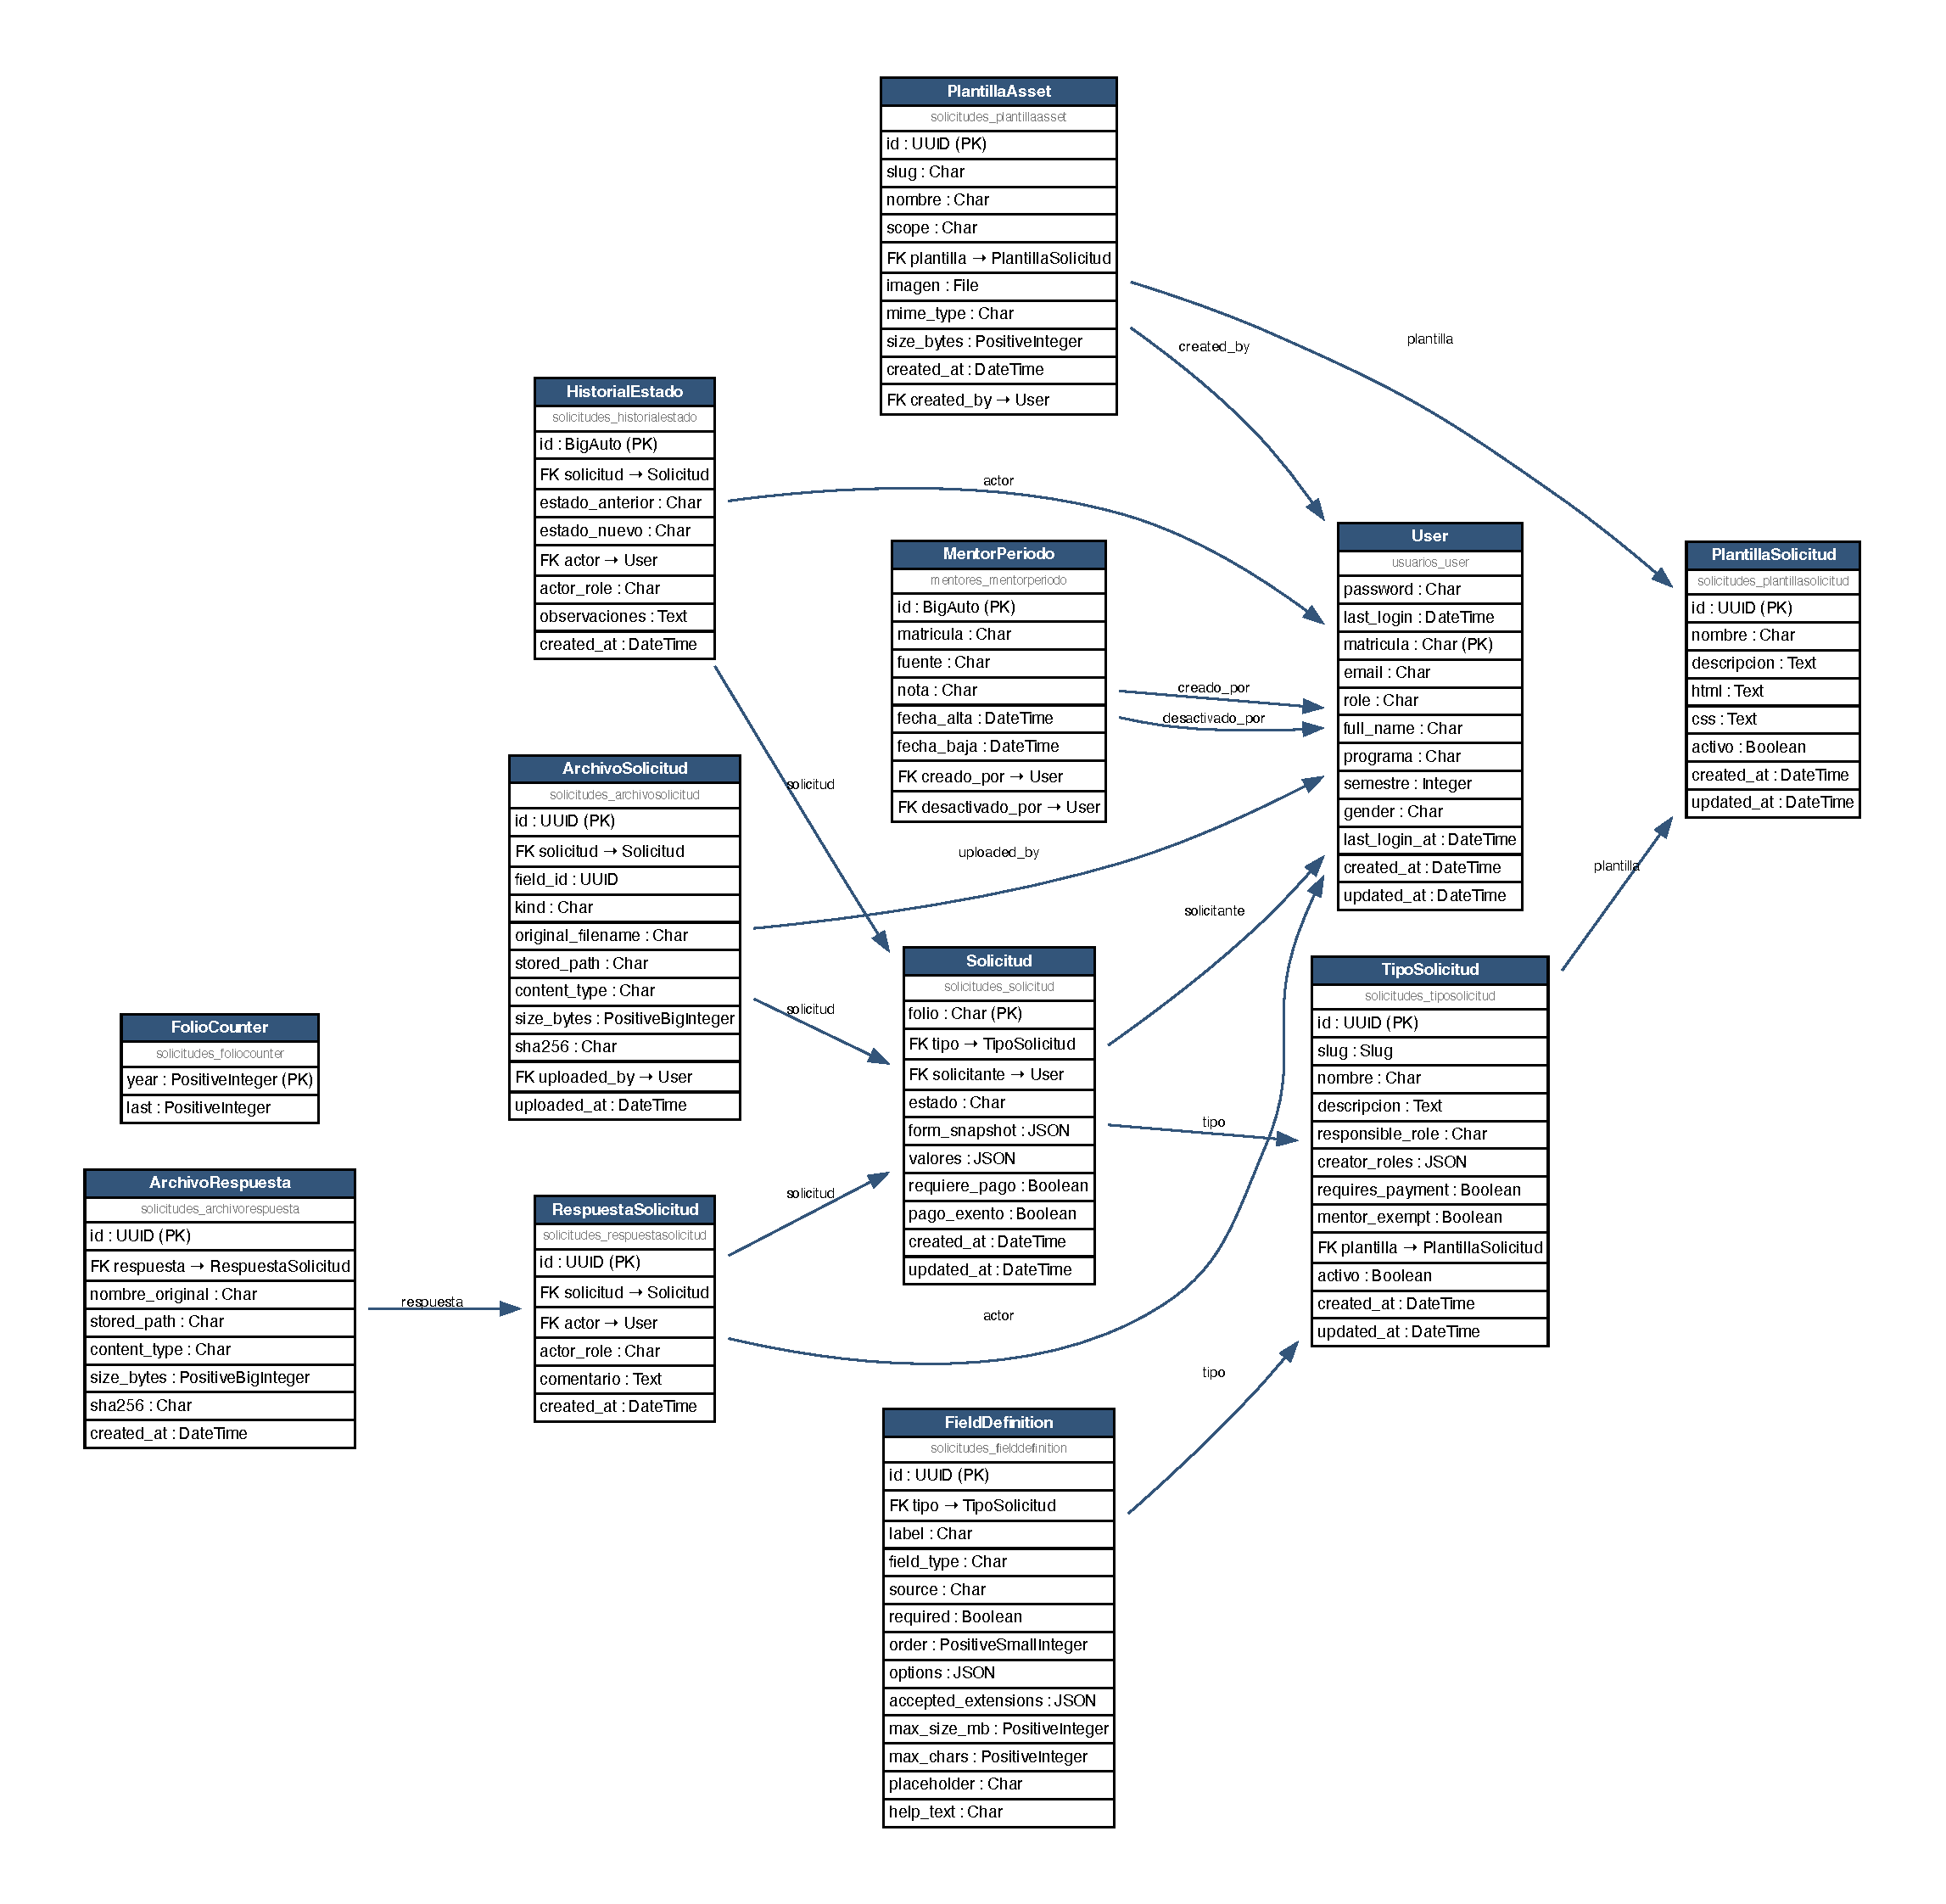
\includegraphics[width=\textwidth]{../esquema_bd_diagrama.pdf}
\caption{Diagrama entidad-relación del Sistema de Solicitudes.}
\label{fig:er}
\end{figure}

\section{Entidades clave}

\begin{description}[leftmargin=0em, style=nextline]
  \item[\texttt{User} (usuarios)] Llave primaria \texttt{matricula}. Campos:
  \texttt{email} (único, propiedad del proveedor de auth), \texttt{role},
  campos cacheados de SIGA (\texttt{full\_name}, \texttt{programa},
  \texttt{semestre}, \texttt{gender}), \texttt{last\_login\_at} y auditoría. Las
  cadenas vacías nunca sobrescriben valores cacheados (contrato de re-\textit{login}
  con solo JWT).

  \item[\texttt{TipoSolicitud} (solicitudes)] \texttt{id} (UUID), \texttt{slug}
  único, \texttt{nombre}, \texttt{descripcion}, \texttt{responsible\_role},
  \texttt{creator\_roles} (JSON), \texttt{requires\_payment},
  \texttt{mentor\_exempt}, \texttt{plantilla} (FK a \texttt{PlantillaSolicitud},
  \texttt{SET\_NULL}), \texttt{activo} y auditoría.

  \item[\texttt{FieldDefinition} (solicitudes)] \texttt{id} (UUID), \texttt{tipo}
  (FK CASCADE), \texttt{label}, \texttt{field\_type}, \texttt{required},
  \texttt{order} (único por tipo), \texttt{options} (SELECT),
  \texttt{accepted\_extensions} / \texttt{max\_size\_mb} (FILE),
  \texttt{max\_chars} (TEXT/TEXTAREA), \texttt{source} (auto-llenado).

  \item[\texttt{Solicitud} (solicitudes)] Llave primaria \texttt{folio}
  (\texttt{SOL-AAAA-NNNNN}). Campos: \texttt{tipo} (FK PROTECT),
  \texttt{solicitante} (FK PROTECT), \texttt{estado},
  \texttt{form\_snapshot} (JSON, congelado al crear), \texttt{valores} (JSON),
  \texttt{requiere\_pago}, \texttt{pago\_exento} y auditoría.

  \item[\texttt{HistorialEstado} (solicitudes)] \texttt{id}, \texttt{solicitud}
  (FK CASCADE), \texttt{estado\_anterior} (nulo en el alta), \texttt{estado\_nuevo},
  \texttt{actor} (FK PROTECT), \texttt{actor\_role} (\textit{snapshot}),
  \texttt{observaciones}, \texttt{created\_at}. De solo anexado.

  \item[\texttt{FolioCounter} (solicitudes)] \texttt{year} (PK), \texttt{last}.
  Una fila por año; \texttt{select\_for\_update} serializa la asignación.

  \item[\texttt{ArchivoSolicitud} (solicitudes)] \texttt{id} (UUID),
  \texttt{solicitud} (FK CASCADE), \texttt{field\_id} (UUID, nulo para
  comprobante), \texttt{kind} (FORM/COMPROBANTE), \texttt{original\_filename},
  \texttt{stored\_path}, \texttt{content\_type}, \texttt{size\_bytes},
  \texttt{sha256}, \texttt{uploaded\_by} (FK PROTECT). Restricciones parciales de
  unicidad por \texttt{(solicitud, field\_id)} y por comprobante.

  \item[\texttt{PlantillaSolicitud} (solicitudes)] \texttt{id} (UUID),
  \texttt{nombre}, \texttt{descripcion}, \texttt{html} (cuerpo de plantilla
  Django), \texttt{css}, \texttt{activo} y auditoría.

  \item[\texttt{PlantillaAsset} (solicitudes)] \texttt{id} (UUID), \texttt{slug},
  \texttt{nombre}, \texttt{scope} (global/plantilla), \texttt{plantilla} (FK
  CASCADE, nulo si global), \texttt{imagen}, \texttt{mime\_type},
  \texttt{size\_bytes}, \texttt{created\_by} (FK PROTECT). Unicidad de \texttt{slug}
  por alcance y \textit{check} de consistencia de alcance.

  \item[\texttt{RespuestaSolicitud} (solicitudes)] \texttt{id} (UUID),
  \texttt{solicitud} (FK CASCADE), \texttt{actor} (FK PROTECT),
  \texttt{actor\_role} (\textit{snapshot}), \texttt{comentario},
  \texttt{created\_at}. Es el \emph{lote} de respuesta.

  \item[\texttt{ArchivoRespuesta} (solicitudes)] \texttt{id} (UUID),
  \texttt{respuesta} (FK CASCADE), \texttt{nombre\_original},
  \texttt{stored\_path}, \texttt{content\_type}, \texttt{size\_bytes},
  \texttt{sha256}, \texttt{created\_at}. Un archivo de un lote.

  \item[\texttt{MentorPeriodo} (mentores)] \texttt{id} (BigAuto),
  \texttt{matricula} (indexada), \texttt{fuente} (MANUAL/CSV), \texttt{nota},
  \texttt{fecha\_alta}, \texttt{fecha\_baja} (nulo = periodo abierto),
  \texttt{creado\_por} y \texttt{desactivado\_por} (FK PROTECT). Unicidad parcial:
  un único periodo abierto por matrícula.
\end{description}

\section{Integridad y consistencia}

\begin{itemize}[leftmargin=1.4em]
  \item \textbf{Inmutabilidad del \textit{snapshot}.} \texttt{Solicitud.form\_snapshot},
  \texttt{requiere\_pago} y \texttt{pago\_exento} se congelan al crear y no se
  recalculan al leer, de modo que la auditoría y los reportes son estables aunque
  el tipo o la lista de mentores cambien después.
  \item \textbf{Borrado protegido.} Las relaciones a \texttt{User} y a
  \texttt{TipoSolicitud} usan \texttt{PROTECT} para impedir borrados que
  huérfanen historial o solicitudes.
  \item \textbf{Solo anexado.} \texttt{HistorialEstado} y las respuestas no
  exponen métodos de borrado o actualización en sus repositorios.
\end{itemize}

% =====================================================================
\chapter{Decisiones de diseño y patrones}
% =====================================================================

\section{DTOs de Pydantic en las fronteras}

Cada cruce de capa transporta un DTO inmutable (\texttt{frozen=True}). Esto
desacopla la representación de persistencia (modelos ORM) de la representación de
dominio y de presentación, evita que el ORM se filtre a las plantillas y permite
validar invariantes en el punto de construcción del DTO mediante validadores de
Pydantic (\texttt{@model\_validator}).

\section{Inyección de dependencias por funcionalidad}

Cada funcionalidad declara su grafo de dependencias en \texttt{dependencies.py}
mediante \emph{funciones de fábrica} (p.\,ej.
\texttt{get\_intake\_service()}). Las vistas llaman a la fábrica una vez por
petición. Esto mantiene a los servicios libres de framework, facilita las
pruebas (se inyectan repositorios falsos en memoria) y resuelve ciclos de
construcción —por ejemplo, el ciclo entre \texttt{LifecycleService} y
\texttt{NotificationService} se rompe construyendo una instancia de ciclo de vida
de solo lectura con un notificador \texttt{NoOp} para el notificador.

\section{Máquina de estados del ciclo de vida}

El ciclo de vida de una solicitud se modela como un mapa explícito de
transiciones legales:

\begin{table}[H]
\centering
\caption{Transiciones legales de \texttt{Solicitud.estado}.}
\begin{tabularx}{\textwidth}{L{3.6cm} L{2.8cm} L{3.6cm} X}
\toprule
\textbf{Estado origen} & \textbf{Acción} & \textbf{Estado destino} & \textbf{Quién} \\
\midrule
CREADA      & atender    & EN\_PROCESO  & Personal del rol responsable / admin \\
EN\_PROCESO & finalizar  & FINALIZADA   & Personal del rol responsable / admin \\
CREADA      & cancelar   & CANCELADA    & Solicitante (dueño), personal, admin \\
EN\_PROCESO & cancelar   & CANCELADA    & Personal del rol responsable / admin \\
\bottomrule
\end{tabularx}
\end{table}

Las transiciones prohibidas elevan \texttt{InvalidStateTransition} (409). Cada
transición exitosa escribe un \texttt{HistorialEstado} (actor, rol, fecha,
observaciones) y emite una notificación. Reglas de cancelación: el solicitante
solo en \texttt{CREADA}; el personal del rol responsable desde \texttt{CREADA} o
\texttt{EN\_PROCESO}; el administrador desde cualquier estado no terminal. La cola
es \emph{compartida} (no hay campo \texttt{assigned\_to}); gana la primera
escritura ante contención.

\section{Folios únicos}

\texttt{FolioCounter} mantiene una fila por año. \texttt{OrmFolioRepository.allocate}
usa \texttt{select\_for\_update} dentro de una transacción para serializar la
asignación e incrementar el contador; \texttt{DefaultFolioService.next\_folio}
formatea \texttt{SOL-\{year\}-\{n:05d\}}. El \textit{throughput} queda acotado por
la contención de bloqueo a nivel de fila, lo cual es suficiente para el perfil de
carga del proyecto.

\section{Generación de PDF con WeasyPrint}

\texttt{\_shared/pdf.render\_pdf} es la única superficie de WeasyPrint del
sistema. El \texttt{PdfService} compone los datos de la solicitud, el solicitante
y la plantilla, construye el contexto de render, evalúa el cuerpo de la plantilla
como plantilla de Django y produce los bytes. No se persiste el PDF: cada
descarga re-renderiza desde el origen, garantizando consistencia con el estado
actual. El \texttt{pdf\_identifier} combinado con un reloj fijo produce bytes
idénticos para la misma entrada (determinismo dentro de un entorno). Las imágenes
se incrustan como URIs \texttt{data:} para estabilidad entre despliegues.

\section{Almacenamiento de archivos transaccional}

\texttt{LocalFileStorage.save} escribe los bytes en un archivo \texttt{.partial}
y registra un \textit{hook} \texttt{transaction.on\_commit} que renombra
atómicamente a la ruta final con \texttt{os.replace}. Si la transacción externa
revierte, el \textit{hook} no se dispara y el \texttt{.partial} se limpia con
\texttt{cleanup\_pending()}. Esto evita huérfanos y archivos sin fila. La ruta se
resuelve contra \texttt{MEDIA\_ROOT} rechazando rutas que escapen de la raíz.

\section{Auditoría}

\texttt{audit.write(event, **fields)} emite una línea INFO estructurada en el
\textit{logger} \texttt{audit} con los campos relevantes (sin persistencia en
base de datos en la versión 1; el flujo de \textit{logs} JSON es la superficie
consultable). Se invoca en \texttt{solicitud.creada} y
\texttt{solicitud.estado\_cambiado}, fuera de la transacción, como observabilidad
de mejor esfuerzo.

% =====================================================================
\chapter{Diseño de interfaz de usuario}
% =====================================================================

\section{Distribución general}

La interfaz se renderiza en el servidor con Django Templates, estilizada con
Tailwind CSS v4 (enfoque \textit{CSS-first} mediante \texttt{@theme}), con
interactividad ligera mediante Alpine.js v3 e iconos de Lucide. Existe una
plantilla base (\texttt{base.html}) con una barra lateral
(\texttt{components/sidebar.html}) cuyas secciones se muestran según el rol del
usuario, y un área de contenido principal. La estética sigue las convenciones del
\textit{skill} \texttt{frontend-design}: aspecto profesional e institucional,
accesible (WCAG 2.2 AA) y localizado a español de México.

\section{Componentes compartidos}

Bajo \texttt{templates/solicitudes/\_partials/} viven parciales reutilizados
entre las vistas de solicitante y de personal: la insignia de estado
(\texttt{\_estado\_badge.html}, que comunica el estado por color \emph{y} texto
para cumplir WCAG), la fila de solicitud, la línea de tiempo del historial, el
renderizado de valores del \textit{snapshot}, el listado de archivos y el listado
de respuestas. La reutilización garantiza coherencia visual entre intake y
revision.

\section{Vistas por rol}

\begin{table}[H]
\centering
\caption{Superficies principales de la interfaz según el rol.}
\begin{tabularx}{\textwidth}{L{3.4cm} X}
\toprule
\textbf{Rol} & \textbf{Vistas principales} \\
\midrule
Alumno / Docente & Catálogo de tipos, alta de solicitud (formulario dinámico),
``Mis solicitudes'' (lista filtrable), detalle con historial y documentos de
respuesta. \\
Control Escolar / Resp. de Programa & Cola compartida por rol, detalle con
acciones (atender / finalizar / cancelar), adjuntar respuesta. \\
Administrador & CRUD de tipos y plantillas, biblioteca de imágenes, catálogo de
mentores, directorio de usuarios, tablero de reportes y exportaciones. \\
\bottomrule
\end{tabularx}
\end{table}

\section{Accesibilidad y diseño responsivo}

Las plantillas incluyen \textit{skip-link}, un único \texttt{h1} por página,
tablas con columnas de baja prioridad ocultas en pantallas estrechas, estados
comunicados por color y texto, y reflujo verificado a 320~px. Los formularios
marcan los campos requeridos y exponen los errores con \texttt{role="alert"}.

% =====================================================================
\chapter{Seguridad}
% =====================================================================

\section{Autenticación delegada (JWT)}

El sistema no gestiona credenciales: recibe un JWT de un proveedor externo
(RNF-01, RT-01). El \texttt{JwtAuthenticationMiddleware} lee la cookie
\texttt{stk} (o la cabecera \texttt{Authorization: Bearer}), valida la firma y la
expiración con \texttt{\_shared.auth.decode\_jwt}, y fija \texttt{request.user} y
\texttt{request.user\_dto}. Ante un token inválido o expirado redirige al
\textit{login} externo. La cookie \texttt{stk} es \texttt{HttpOnly},
\texttt{SameSite=Lax}, \texttt{Secure} en producción, con \texttt{max\_age}
derivado de la expiración del token.

\section{Autorización en capas}

La autorización se aplica en dos niveles complementarios:

\begin{enumerate}[leftmargin=1.6em]
  \item \textbf{Vista (grueso).} \textit{Mixins} por rol
  (\texttt{CreatorRequiredMixin}, \texttt{ReviewerRequiredMixin},
  \texttt{AdminRequiredMixin}) restringen el acceso a la ruta según el rol.
  \item \textbf{Servicio (política de dominio).} La autorización autoritativa vive
  en el servicio. Por ejemplo, \texttt{LifecycleService.\_authorize} decide quién
  puede invocar cada transición; \texttt{ArchivoService} y
  \texttt{RespuestaService} aplican matrices de visibilidad por rol y estado;
  \texttt{IntakeService} re-verifica que el rol del actor pertenezca a
  \texttt{creator\_roles} (defensa en profundidad sobre el \textit{mixin}).
\end{enumerate}

Las matrices de visibilidad de archivos y respuestas restringen la descarga al
dueño de la solicitud, al personal del rol responsable y al administrador; el
solicitante solo ve los documentos de respuesta cuando la solicitud está
\texttt{FINALIZADA}.

\section{CSP en la previsualización de plantillas}

El editor de plantillas evalúa HTML+CSS suministrado por el administrador. Los
\textit{endpoints} de previsualización renderizan en un \texttt{iframe} con
\texttt{srcdoc} y envían una cabecera \texttt{Content-Security-Policy} estricta
(\texttt{default-src 'none'; style-src 'unsafe-inline'; img-src data: https:
'self'; font-src data:}) más \texttt{X-Frame-Options: SAMEORIGIN}. El
\texttt{iframe} se aísla sin \texttt{allow-scripts}. Estos \textit{endpoints} son
exclusivos de administradores (\texttt{AdminRequiredMixin}); el administrador es
un operador de confianza, y la superficie de plantilla queda acotada por el
aislamiento del \texttt{iframe} y la restricción de rol.

\section{Validación de archivos}

Toda carga se valida por extensión y tamaño (tope global de 10~MB, RT-07) en el
formulario y, de forma autoritativa, en el servicio. Las imágenes de la
biblioteca se verifican adicionalmente con PIL contra los bytes reales para
detectar cargas renombradas; SVG se rechaza explícitamente para evitar
\textit{scripts} embebidos. Las rutas de almacenamiento se resuelven contra
\texttt{MEDIA\_ROOT} rechazando intentos de salir de la raíz.

\section{Transporte y entornos}

Todo el tráfico de navegador pasa por nginx con terminación TLS (TLS 1.2+,
RT-04); en producción se exige TLSv1.3, HSTS, CSP y limitación de tasa. Los
secretos (\texttt{JWT\_SECRET}, credenciales de SMTP, URL de SIGA) se inyectan por
variables de entorno; \texttt{prod.py} falla al arrancar si falta alguno
requerido, evitando despliegues mal configurados.

% =====================================================================
\chapter{Tecnologías y dependencias}
% =====================================================================

\begin{table}[H]
\centering
\caption{Pila tecnológica del Sistema de Solicitudes.}
\begin{tabularx}{\textwidth}{L{4.2cm} X}
\toprule
\textbf{Capa} & \textbf{Tecnología} \\
\midrule
Lenguaje      & Python 3.12+ \\
Framework     & Django 5.x (plantillas en servidor, sin DRF) \\
DTOs          & Pydantic v2 en cada frontera de capa \\
Presentación  & Django Templates + Tailwind CSS v4 + Alpine.js v3 + iconos Lucide \\
Base de datos & PostgreSQL 16 (SQLite solo para el bucle de pruebas en proceso); ORM de Django contenido en repositorios \\
PDF           & WeasyPrint (dependencias de sistema en la imagen) \\
Tareas async  & Ninguna en v1 (correo síncrono con \texttt{try/except}); Celery + Redis diferidos \\
Almacenamiento de archivos & Sistema de archivos local (\texttt{media/}); abstracción \texttt{FileStorage} conmutable \\
Autenticación & Validación de JWT en \textit{middleware} (proveedor externo) \\
Pruebas       & \texttt{pytest} + \texttt{pytest-django}, \texttt{model\_bakery}, \texttt{freezegun}, \texttt{responses}, \texttt{pytest-playwright} \\
Ejecución     & \texttt{Dockerfile} multietapa; \texttt{docker-compose} (nginx, web, db, mailhog); \texttt{Makefile} como punto de entrada \\
Proxy inverso & nginx (TLS); configuraciones separadas para desarrollo y producción \\
\bottomrule
\end{tabularx}
\end{table}

\section{Integraciones externas}

\begin{table}[H]
\centering
\caption{Interfaces externas del sistema.}
\begin{tabularx}{\textwidth}{L{2.2cm} L{3.2cm} L{2.4cm} X}
\toprule
\textbf{ID} & \textbf{Sistema} & \textbf{Dirección} & \textbf{Datos} \\
\midrule
IE-01 & Proveedor JWT & Entrada (HTTPS) & matrícula, correo, rol \\
IE-02 & SIGA          & Salida (REST/HTTPS) & nombre, programa, semestre, correo \\
IE-03 & SMTP          & Salida (SMTP/TLS) & notificaciones por evento \\
\bottomrule
\end{tabularx}
\end{table}

La consulta a SIGA es de mejor esfuerzo con \textit{timeout} (5~s, RNF-02): ante
falla se degrada usando los datos del JWT. El despacho de correo es tolerante a
fallas: una caída de SMTP se registra y absorbe sin afectar la operación de
negocio (RF-07).

\section{Convenciones de construcción}

El \texttt{Makefile} es el punto de entrada único; cada comando se ejecuta a
través de \texttt{docker compose exec web}. Los ajustes se dividen en
\texttt{config/settings/\{base,dev,prod,test\_postgres\}.py}, con secretos por
variables de entorno. El ruteo de URL es jerárquico y con espacios de nombres
(proyecto $\rightarrow$ aplicación $\rightarrow$ funcionalidad), p.\,ej.
\texttt{solicitudes:intake:create}.

\end{document}
